\documentclass[main.tex]{subfiles}

\begin{document}
\chapter{Parallelisation of electronic-structure calculations\label{ch:optimisation_scf}}

The \texttt{PWscf} (Plane-Wave Self-Consistend Field) package is one of the core modules of \QE, as many other modules need ground state density and total energy as input.
This chapter deals with examining the best ways to run \texttt{PWscf} calculations in the \texttt{scf} mode.

\section{First scaling tests}\label{sec:scf_first_scaling}

The first step in analysing the scaling of the \texttt{PWscf} module is to perform a baseline scaling test without any optimisations appplied. 
In Fig. \ref{fig:scaling_scf_ompi_nprocs_si_speedup} to \ref{fig:scaling_scf_ompi_nprocs_tas2_absolute_wait} two scaling tests on the earlier mentioned benchmarking systems Si and TaS2 are pictured. 
The tests are run using \QE 7.0, compiled using the Fortran and C compilers in \gls{openmpi} 4.1.0, without any of the compilation or runtime optimisation parameters mentioned in section \ref{sec:qe} used.

\begin{figure}[ht!]
\centering
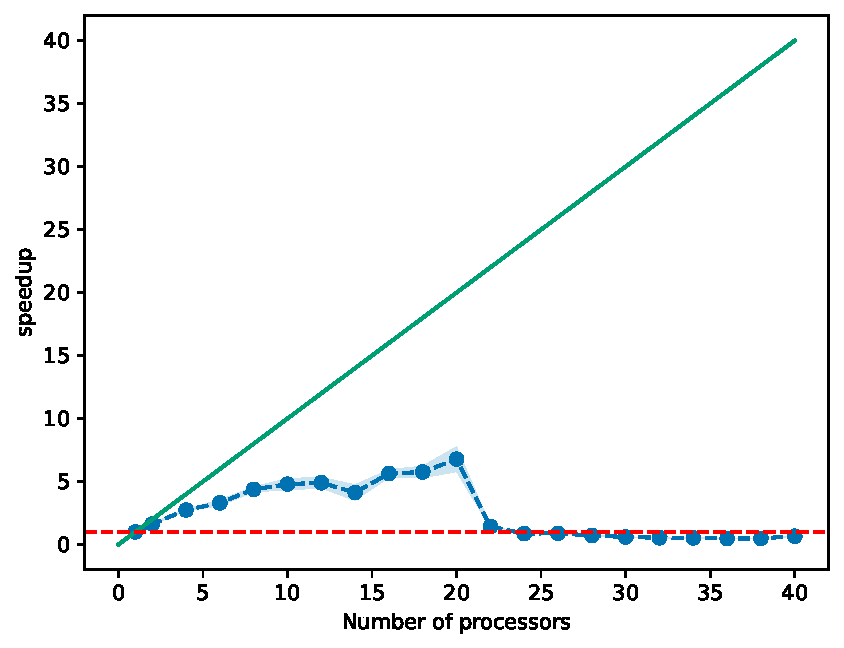
\includegraphics[width=0.75\textwidth]{plots_scf/si_ompi_bench_nprocs_speedup.pdf}
\caption{Baseline scaling test on the Si benchmarking system \emph{\QE 7.0, \gls{openmpi} 4.1.0, \texttt{nk 1} and \texttt{nd 1}}}
\label{fig:scaling_scf_ompi_nprocs_si_speedup}
\end{figure}

\begin{figure}[ht!]
\begin{subfigure}[b]{0.49\textwidth}
    \centering
    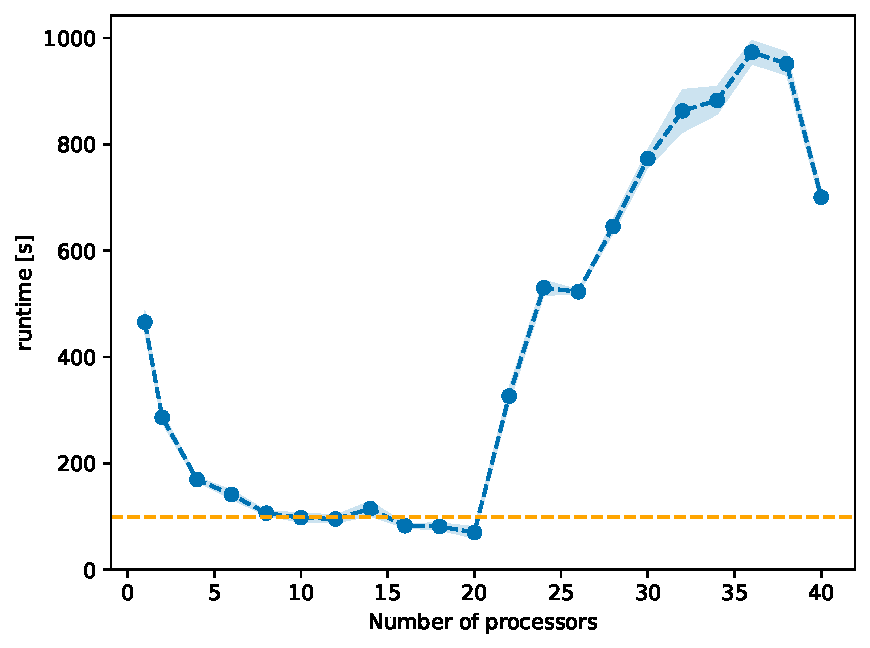
\includegraphics[width=\textwidth]{plots_scf/si_ompi_bench_nprocs_absolute.pdf}
\end{subfigure}
\begin{subfigure}[b]{0.49\textwidth}
    \centering
    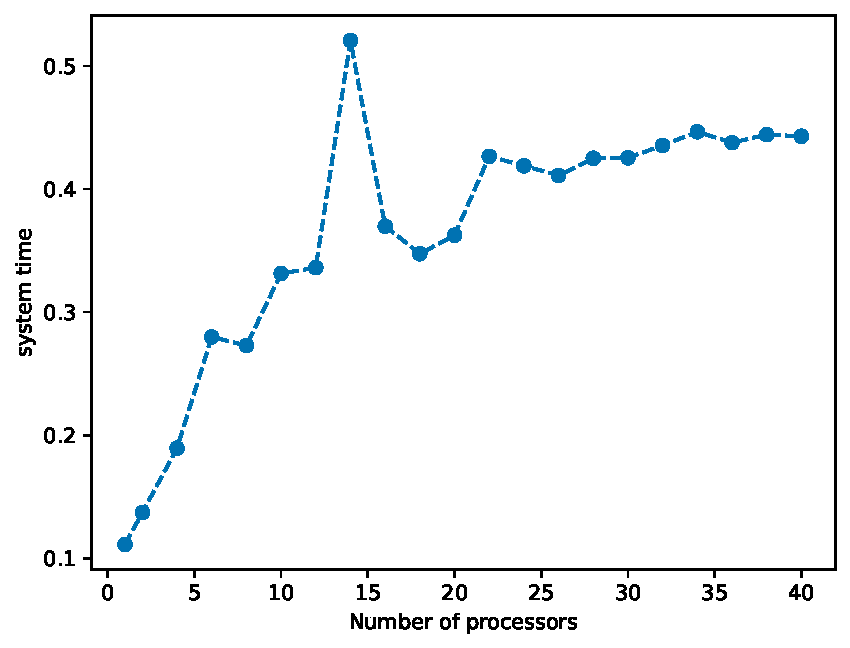
\includegraphics[width=\textwidth]{plots_scf/si_ompi_bench_nprocs_wait.pdf}
\end{subfigure}
\caption{Baseline scaling test on the Si benchmarking system \emph{\QE 7.0, \gls{openmpi} 4.1.0, \texttt{nk 1} and \texttt{nd 1}}}
\label{fig:scaling_scf_ompi_nprocs_si_absolute_wait}
\end{figure}

As discussed in sec. \ref{sub:scalability_qe}, three different metrics of scalability can be deduced from the time data given by \QE:
\begin{itemize}
    \item runtime: absolute runtime (walltime) of the compute job
    \item speedup: runtime divided by runtime of the job on a single core
    \item \gls{wait_time}: percentage of \gls{wall_time} used by system tasks, e.g. writing to disk, etc.
\end{itemize}
These are pictured in fig. \ref{fig:scaling_scf_ompi_nprocs_si_speedup} and \ref{fig:scaling_scf_ompi_nprocs_si_absolute_wait} for the silicon benchmarking system.

On a single node, the speedup does scale linearly with the number of processors until around 10 processors, but with a slope of \(\frac{1}{2}\) instead of 1 (which would mean ideal scaling).
Beyond that number, the slope decreases even more so that a maximal speedup of around 7 is achieved for 20 processors used.
As discussed in sec. \ref{sec:hardware_physnet}, one node is equipped with 20 cores, so trying to scale the communication intensive calculations beyond that threshold makes the calculations run even slower than on a single core.
Interestingly, the wait time plot in \ref{fig:scaling_scf_ompi_nprocs_si_absolute_wait} shows that a significant amount (\(\SI{10}{\percent}\) to \(\SI{40}{\percent}\)) of runtime is taken up by wait time already for less than 20 processors.
As discussed in sec. \ref{sub:scalability_general}, this hints to poor parallelization, which is a reason for the poor scaling seen in fig. \ref{fig:scaling_scf_ompi_nprocs_si_speedup}.

Pictured in fig. \ref{fig:scaling_scf_ompi_nprocs_tas2_speedup} and \ref{fig:scaling_scf_ompi_nprocs_tas2_absolute_wait} are the same scaling test run for the TaS2 benchmarking system.

\begin{figure}[ht!]
\centering
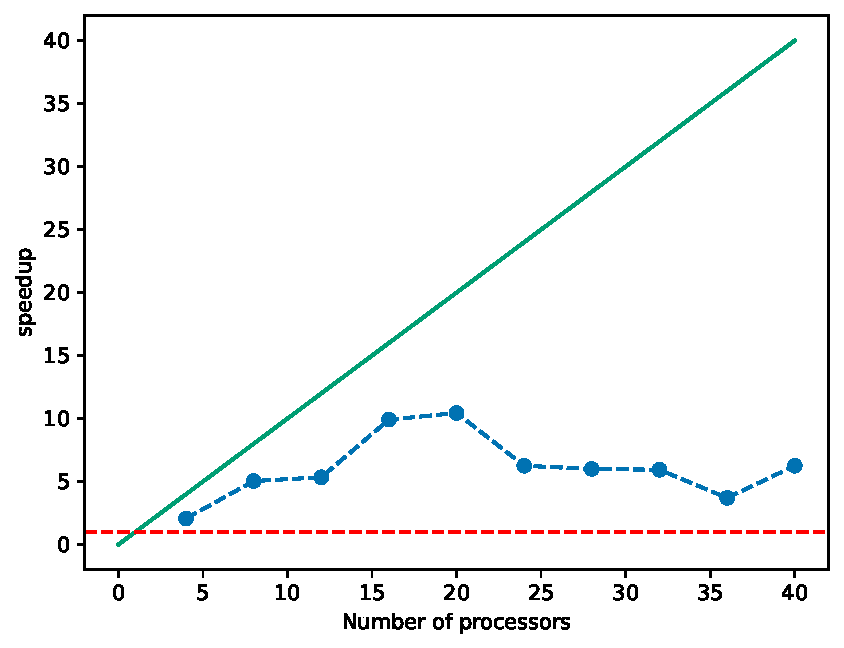
\includegraphics[width=0.75\textwidth]{plots_scf/TaS2_ompi_bench_nprocs_speedup.pdf}
\caption{Baseline scaling test on the TaS2 benchmarking system \emph{\QE 7.0, OpenMPI 4.1.0, \texttt{nk 1} and \texttt{nd 1}}}
\label{fig:scaling_scf_ompi_nprocs_tas2_speedup}
\end{figure}

\begin{figure}[ht!]
\begin{subfigure}[b]{0.49\textwidth}
    \centering
    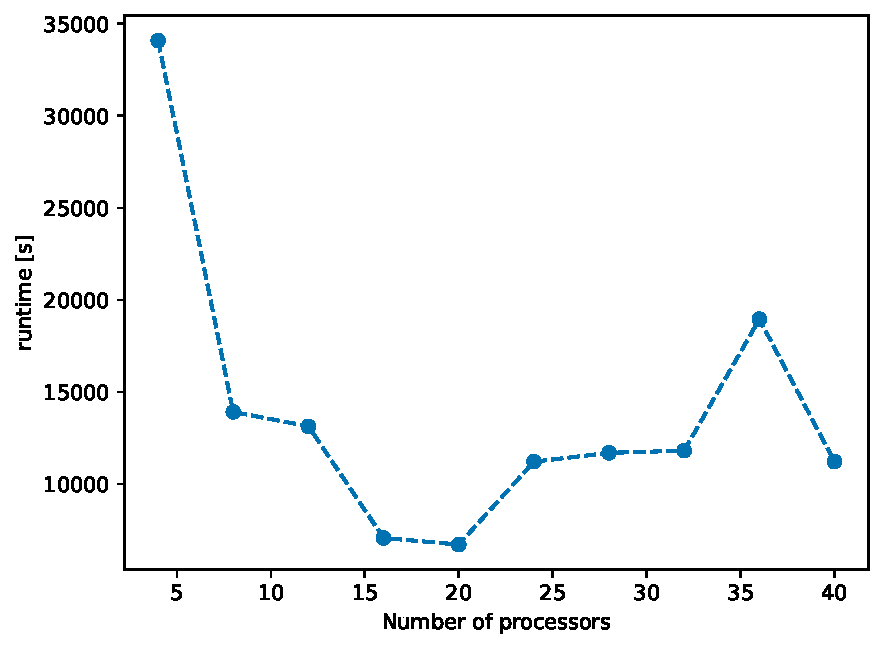
\includegraphics[width=\textwidth]{plots_scf/TaS2_ompi_bench_nprocs_absolute.pdf}
\end{subfigure}
\begin{subfigure}[b]{0.49\textwidth}
    \centering
    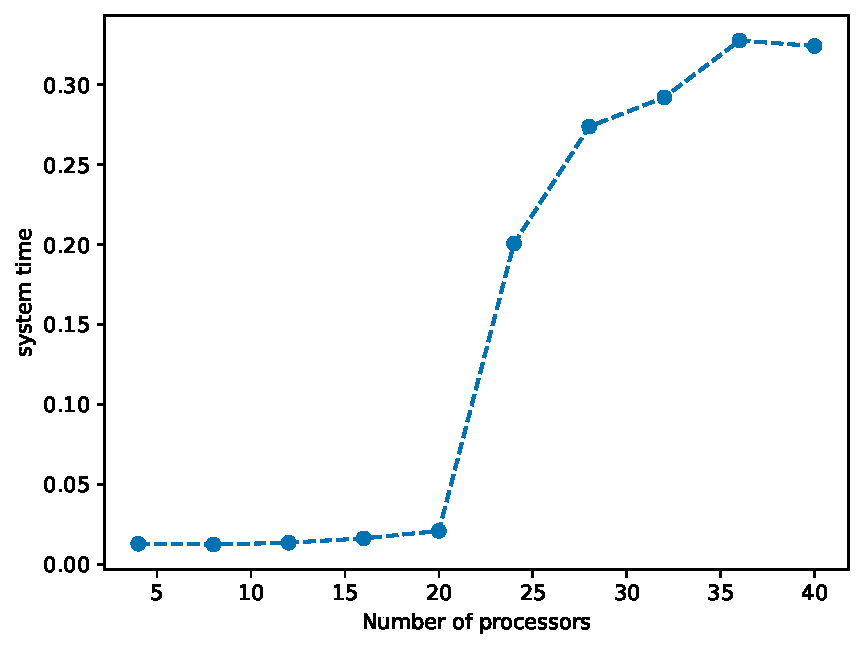
\includegraphics[width=\textwidth]{plots_scf/TaS2_ompi_bench_nprocs_wait.pdf}
\end{subfigure}
\caption{Baseline scaling test on the TaS2 benchmarking system \emph{\QE 7.0, OpenMPI 4.1.0, \texttt{nk 1} and \texttt{nd 1}}}
\label{fig:scaling_scf_ompi_nprocs_tas2_absolute_wait}
\end{figure}
Both benchmarks share a key feature in the linear scaling in speedup with a slope of \(\frac{1}{2}\) up to 10 processors, the tests on TaS2 actually continue this trend up until 20 processors, resulting in a maximal speedup of 10.
Beyond 20 processors the scaling also gets worse, but there still is a speedup of 2 to 3.
Looking at the wait time plot in fig. \ref{fig:scaling_scf_ompi_nprocs_tas2_absolute_wait} shows the quality of parallelization: for up to 20 processors, the wait time is independent of the number of processors, which is the unavoidable startup overhead for tasks like data distribution.
After that, the wait time scales with the number of processors, which hints to communication being a factor limiting speedup here as discussed in sec. \ref{sub:scalability_general}.

In conclusion, systems with more electrons and by extension bigger matrices and longer iteration times seem to be parallelize better and as such profit more from using more processors than systems with just a few number of electrons.

These scaling tests pose now two questions to be answered:
\begin{itemize}
    \item Is better scaling on a single node possible?
    \item How can acceptable scaling over more than one node be achieved?
\end{itemize}

\section{Testing different compilers and mathematical libraries}

A first strategy for solving issues with parallelization is trying different compilers and mathematical libraries.
As discussed in sec. \ref{sub:qe_compilation}, \QE can make use of a variety of software packages available on the PHYSnet cluster.
The benchmarks in \ref{fig:scaling_scf_compilers_nprocs} are run with the following software combinations:
\begin{itemize}
    \item \gls{openmpi} 4.1.0 and \QE provided \gls{blas}/\gls{lapack}, so the baseline test discussed in sec. \ref{sec:scf_first_scaling}
    \item \gls{openmpi} 4.1.0, \gls{openblas} 0.3.20 and \gls{scalapack} 2.2.0
    \item \gls{oneapi} 2021.4
\end{itemize}

\begin{figure}[ht!]
\begin{subfigure}[b]{0.49\textwidth}
    \centering
    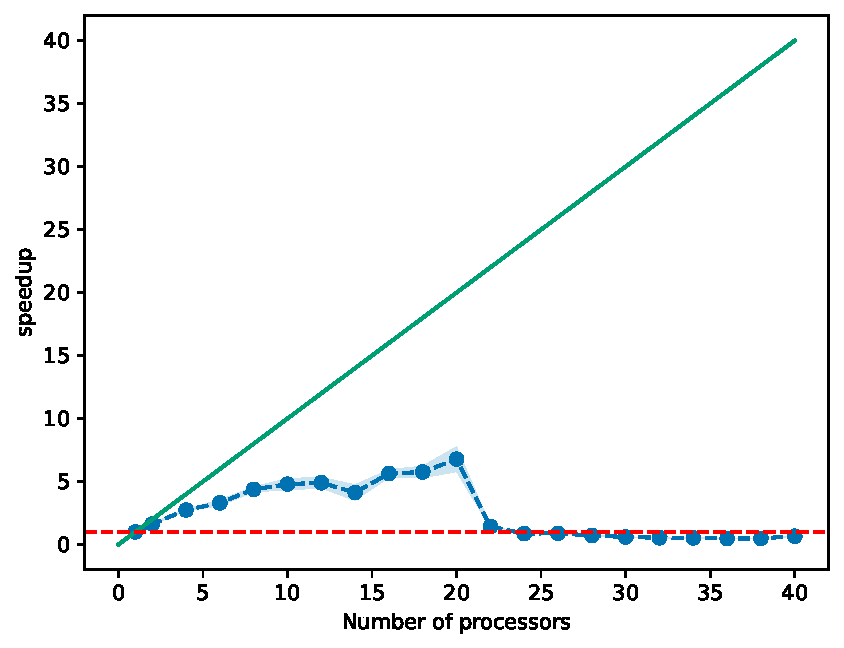
\includegraphics[width=\textwidth]{plots_scf/si_ompi_bench_nprocs_speedup.pdf}
    \subcaption{\gls{openmpi}}
\end{subfigure}
\begin{subfigure}[b]{0.49\textwidth}
    \centering
    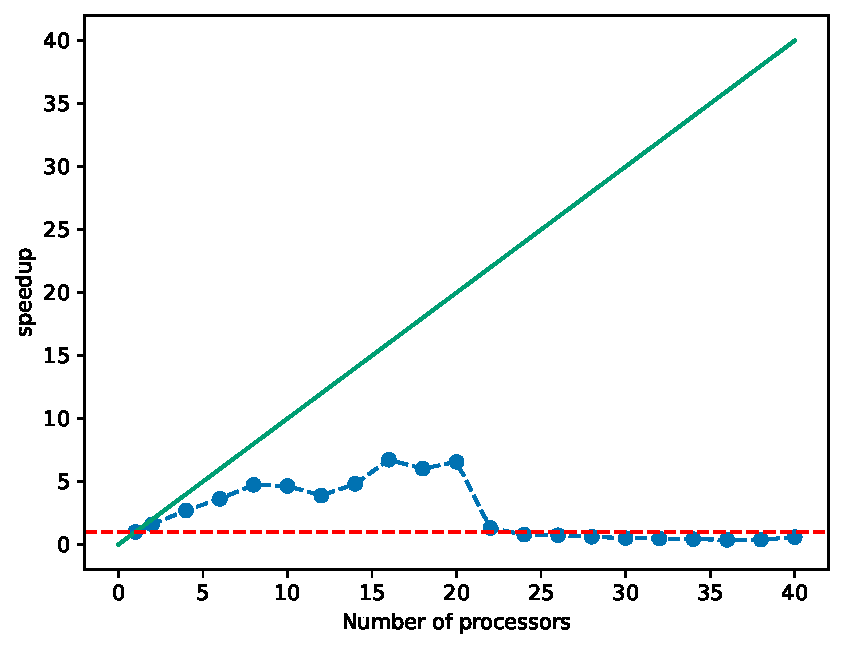
\includegraphics[width=\textwidth]{plots_scf/si_scalapack_bench_nprocs_speedup.pdf}
    \subcaption{\gls{openmpi}, \gls{openblas}, \gls{scalapack}}
\end{subfigure}
\begin{subfigure}[b]{0.49\textwidth}
    \centering
    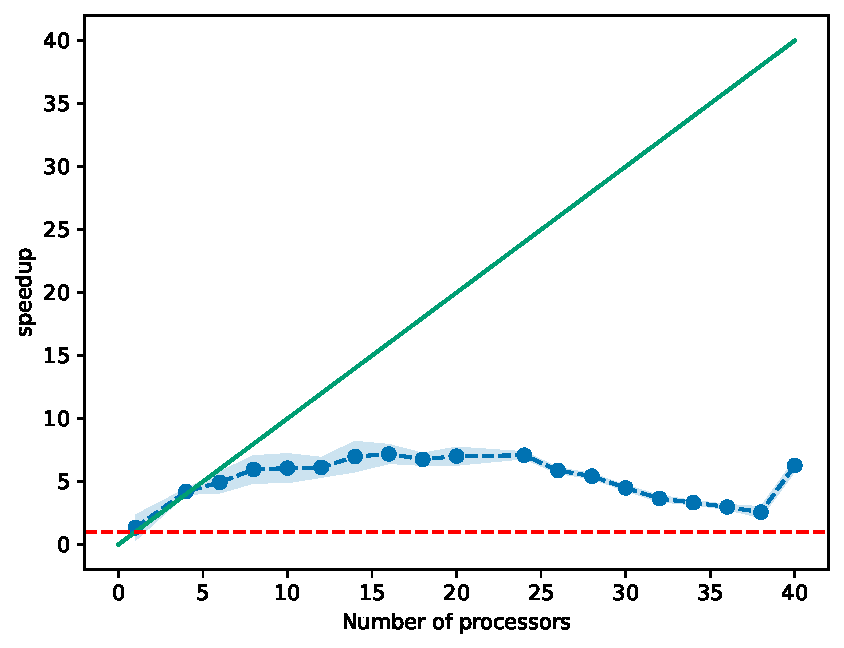
\includegraphics[width=\textwidth]{plots_scf/si_intel_bench_nprocs_speedup.pdf}
    \subcaption{\gls{oneapi}}
\end{subfigure}
\caption{Baseline scaling test Si benchmarking system with different combinations of compilers and mathematical libraries}
\label{fig:scaling_scf_compilers_nprocs}
\end{figure}

Fig. \ref{fig:scaling_scf_compilers_nprocs} shows that just dropping in another \gls{blas} library (\gls{openblas} in this case) does not change the scaling behavior, in contrast to using Intels \gls{oneapi} packages.
Here, optimal scaling behavior is seen for up to 6 processors, which means those calculations ran about twice as fast as the calculations with just \gls{openmpi}.

\begin{figure}[ht!]
\begin{subfigure}[b]{0.49\textwidth}
    \centering
    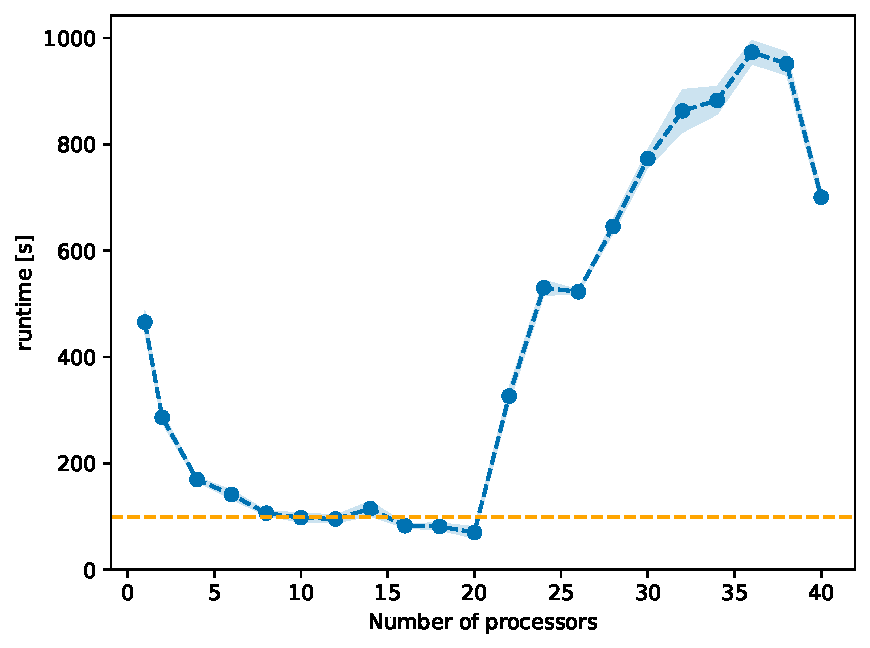
\includegraphics[width=\textwidth]{plots_scf/si_ompi_bench_nprocs_absolute.pdf}
    \subcaption{\gls{openmpi}}
\end{subfigure}
\begin{subfigure}[b]{0.49\textwidth}
    \centering
    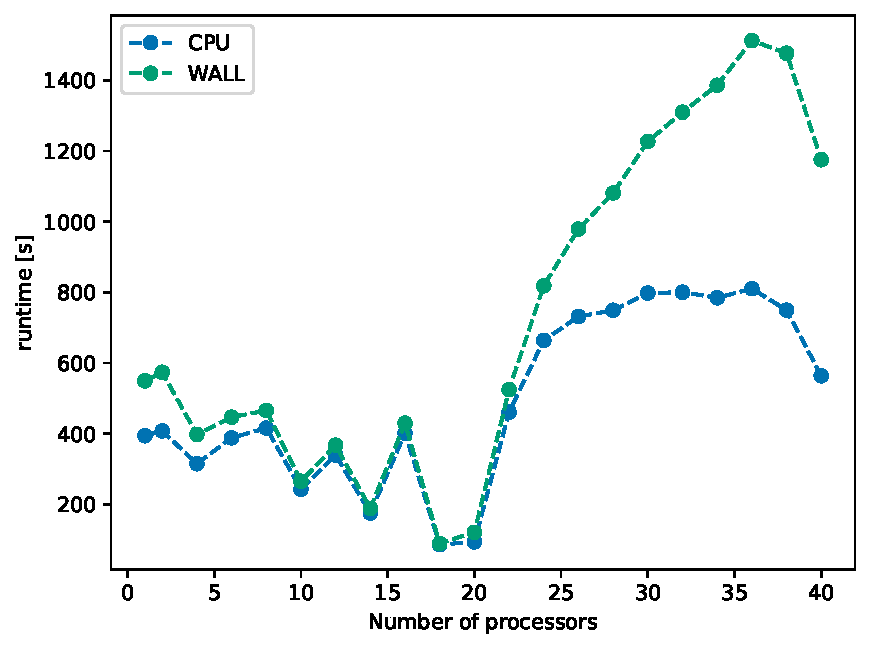
\includegraphics[width=\textwidth]{plots_scf/si_openblas_bench_nprocs_absolute.pdf}
    \subcaption{\gls{openmpi} + \gls{openblas}}
\end{subfigure}
\begin{subfigure}[b]{0.49\textwidth}
    \centering
    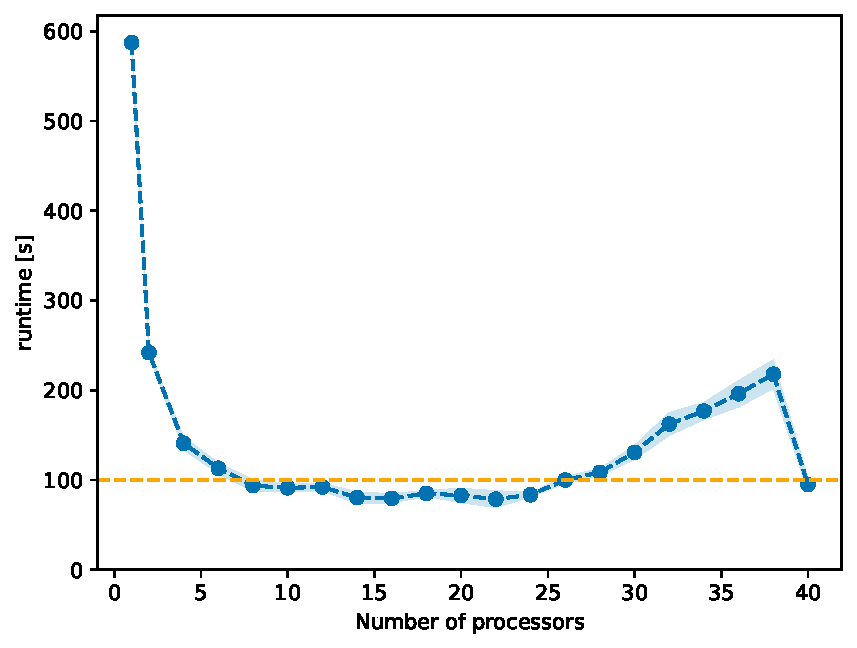
\includegraphics[width=\textwidth]{plots_scf/si_intel_bench_nprocs_absolute.pdf}
    \subcaption{\gls{oneapi}}
\end{subfigure}
\caption{Baseline scaling test Si benchmarking system with different combinations of compilers and mathematical libraries}
\label{fig:scaling_scf_runtime_compilers_nprocs}
\end{figure}

\todo{analyse absolute runtime -> speedup can be deceiving}

\todo{why intel? seems to work best with the infiniband hardware, absolute runtime faster for like 2-4 processors? -> can hint to better perfomance with k point parallelization}

Fig. \ref{fig:scaling_scf_runtime_compilers_nprocs} shows 

\todo{efficiency maybe?}


This result not only stands for itself as a statement about scaling on a single node, but also provides a basis for scaling beyond this apparent optimal range of 6 processors:
The k point parallelization explained in sec. \ref{sub:qe_parallelization} can distribute the workload in such a way that processor pools of sizes within this range work on individual k points and as such can provide optimal scaling within one pool while also not losing performance because the pools do not need to communicate with each other in the same order of magnitude as the pools have to communicate within themselves.

\todo{TaS2 intel scaling?}

\section{Using the parallelization parameters of \QE}

As detailed in section \ref{sub:qe_parallelization}, \QE offers ways to manage how the workload is distributed among the processors.
In \texttt{pw.x} the default plane wave parallelization, k-point-parallelization and linear-algebra parallelization are implemented.

\subsection{k point parallelization}

The benchmark pictured in \ref{fig:scaling_scf_nk_si} is set up as follows: for a given number of processors \(N_p\), the parameter \(N_k\) splits the \(N_p\) processors into \(N_k\) processors pools.
As the number of processors in one pool has to be a whole number, only certain combinations of \(N_p\) and \(N_k\) are possible, for example \(N_p = 32\) could be split into processor pools of size 2 with \(N_k = 16\), size 8 with \(N_k = 4\) or size 16 with \(N_k = 2\).
This leads to choosing the size of the processor pools as a variable, not the parameter \texttt{nk}.
Fig. \ref{fig:scaling_scf_nk_si} shows the scaling for poolsizes 2, 8 and 16 for \QE being compiled with OpenMPI/Scalapack and Intel oneAPI.
This choice of pool sizes showcases the smallest pool size possibly (namely 2), as well as a bigger pool size with 16, that still gives rise to a few data points over the chosen range of processors.

\begin{figure}[ht!]
\begin{subfigure}[b]{0.49\textwidth}
    \centering
    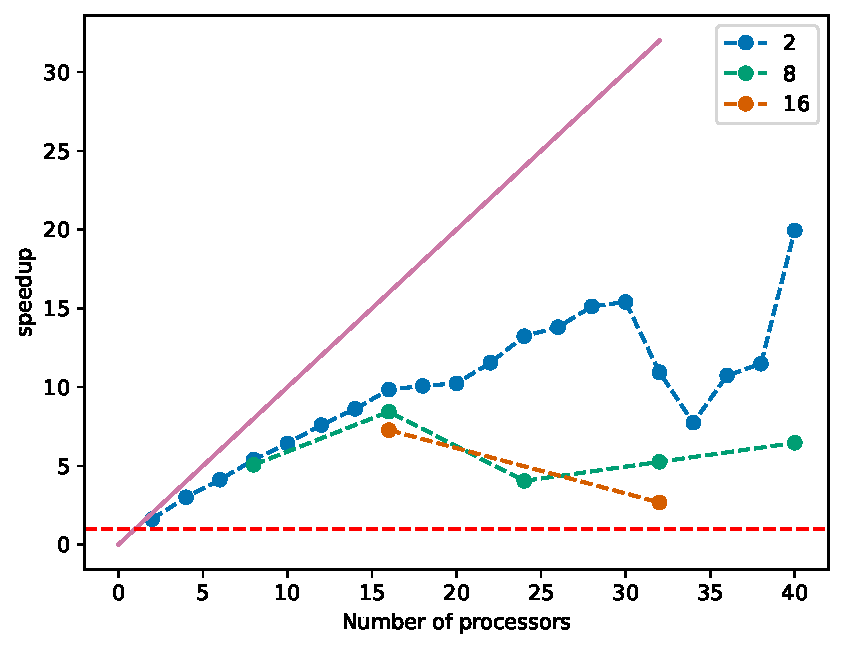
\includegraphics[width=\textwidth]{plots_scf/si_ompi_bench_nk_speedup.pdf}
    \subcaption{\gls{openmpi}}
\end{subfigure}
\begin{subfigure}[b]{0.49\textwidth}
    \centering
    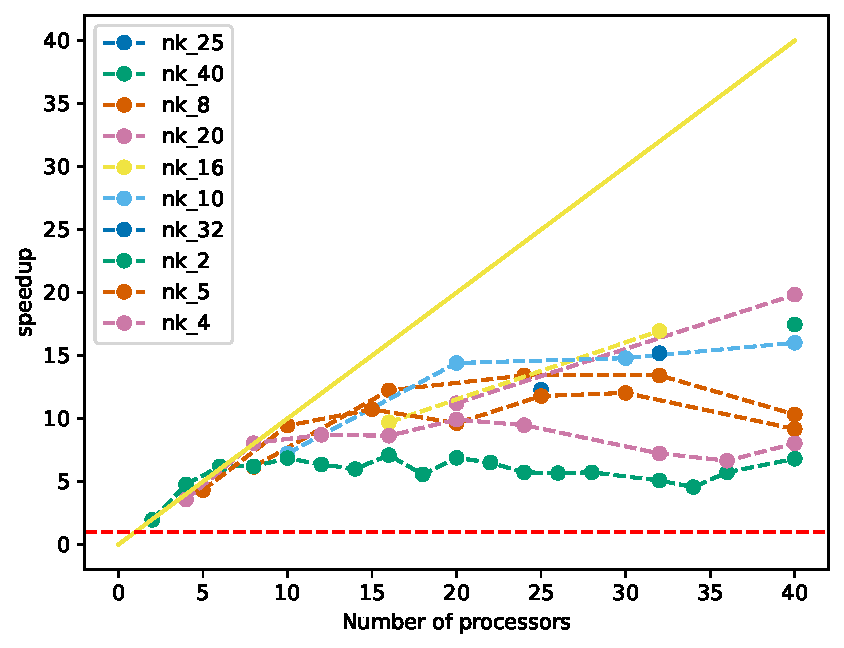
\includegraphics[width=\textwidth]{plots_scf/si_intel_bench_nk_speedup.pdf}
    \subcaption{\gls{oneapi}}
\end{subfigure}
\caption{Benchmark with k-point parallelization for the Si benchmarking system with 3 different sizes of processor pools}
\label{fig:scaling_scf_nk_si}
\end{figure}

Fig. \ref{fig:scaling_scf_nk_si} shows that using k parallelization with a pool size of 2 significantly improves the scaling behavior, not only on one node, but especially over more than one node.

\todo{more analysis: difference between poolsizes}

Another important conclusion to draw out of fig. \ref{fig:scaling_scf_nk_si} is the impact of using Intels compiler instead of OpenMPI, as that factor alone speeds up the calculation by a factor of 2 over the whole range of processors.

\begin{figure}[ht!]
\begin{subfigure}[b]{0.49\textwidth}
    \centering
    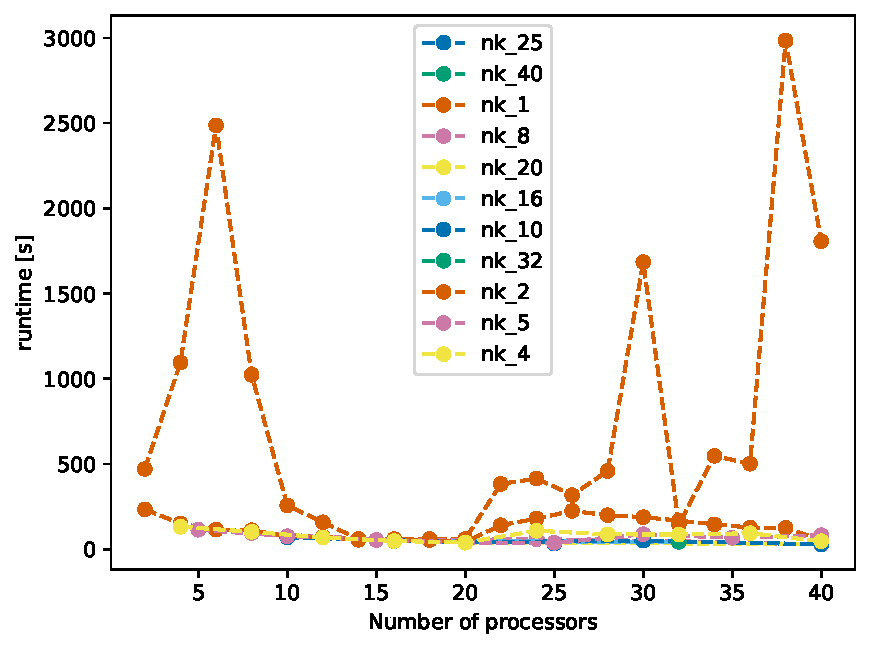
\includegraphics[width=\textwidth]{plots_scf/si_ompi_bench_nk_absolute.pdf}
    \subcaption{\gls{openmpi}}
\end{subfigure}
\begin{subfigure}[b]{0.49\textwidth}
    \centering
    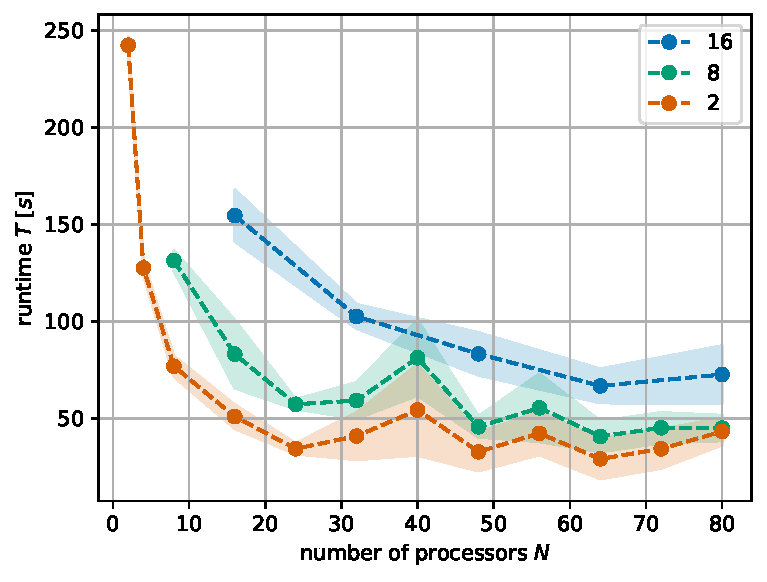
\includegraphics[width=\textwidth]{plots_scf/si_intel_bench_nk_absolute.pdf}
    \subcaption{\gls{oneapi}}
\end{subfigure}
\caption{Benchmark with k-point parallelization for the Si benchmarking system with 3 different sizes of processor pools}
\label{fig:scaling_scf_nk_si_absolute}
\end{figure}

The same scaling test is applied to the TaS2 system in fig. \ref{fig:scaling_scf_nk_tas2}, with a similar list of pool sizes, but over a wider range of processors.

\begin{figure}[ht!]
    \centering
    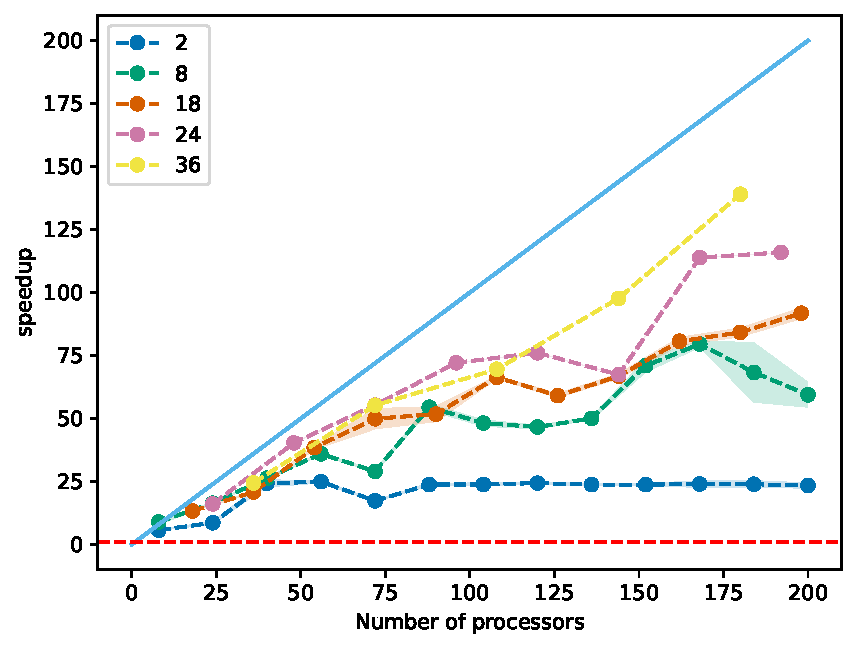
\includegraphics[width=0.8\textwidth]{plots_scf/TaS2_intel_bench_nk_speedup.pdf}
    \caption{Benchmark with k-point parallelization for the TaS2 benchmarking system}
    \label{fig:scaling_scf_nk_tas2}
\end{figure}

Remarkably, the scaling behavior is swapped in comparison to \ref{fig:scaling_scf_nk_si}, as the pool size 2 saturates fast and the bigger pool sizes show way better scaling behavior.
Furthermore, there are instances of better than linear scaling, which according to \QE docs can be attributed to better caching of data.

It can also be instructive to look at the idle time for this benchmark to judge the quality of parallelization. 

\begin{figure}[ht!]
    \centering
    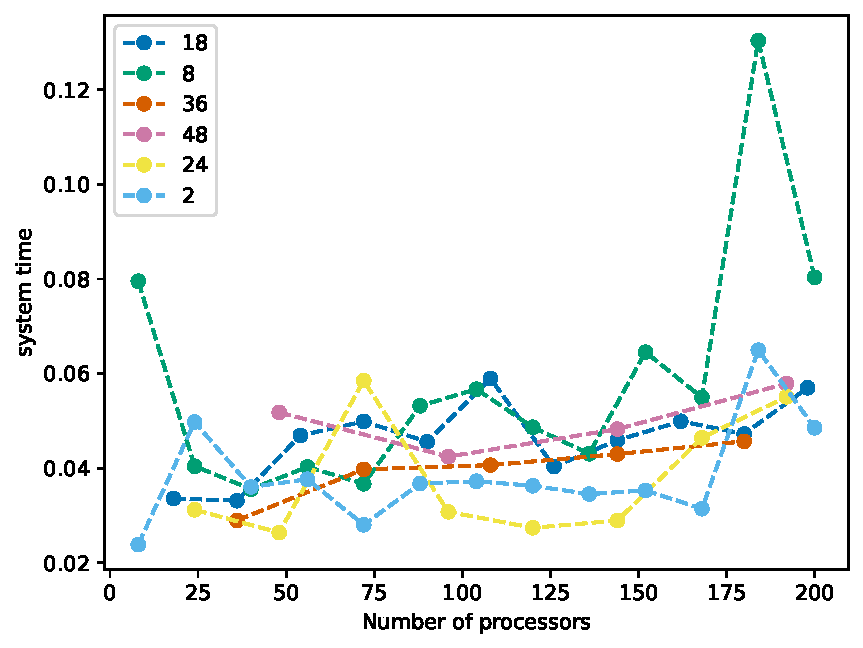
\includegraphics[width=0.8\textwidth]{plots_scf/TaS2_intel_bench_nk_wait.pdf}
    \caption{Idle time for the k point parallelization benchmark for the TaS2 system}
    \label{fig:scaling_scf_nk_tas2_wait}
\end{figure}

Fig. \ref{fig:scaling_scf_nk_tas2_wait} shows a distribution of idle times between about \(\SI{4}{\percent}\) and \(\SI{6}{\percent}\) of the whole \gls{wall_time}, without any kind of systemic increase over any range of processors.
%This means the parallelization is as good as possible for these 
\todo{more analysis: difference between poolsizes}

\subsection{Linear algebra parallelization}

\begin{figure}[ht!]
\begin{subfigure}[b]{0.49\textwidth}
    \centering
    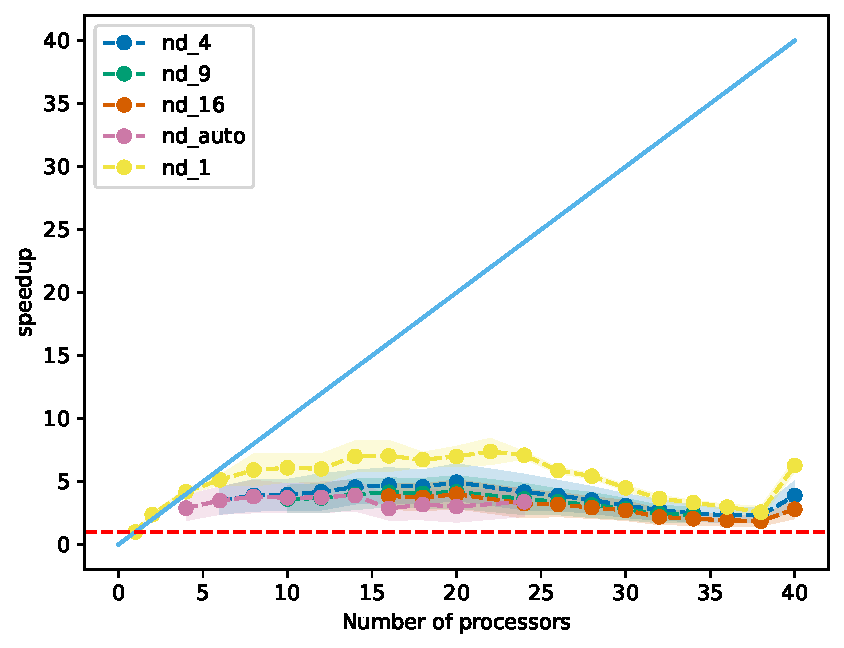
\includegraphics[width=\textwidth]{plots_scf/si_intel_mkl_bench_speedup.pdf}
\end{subfigure}
\begin{subfigure}[b]{0.49\textwidth}
    \centering
    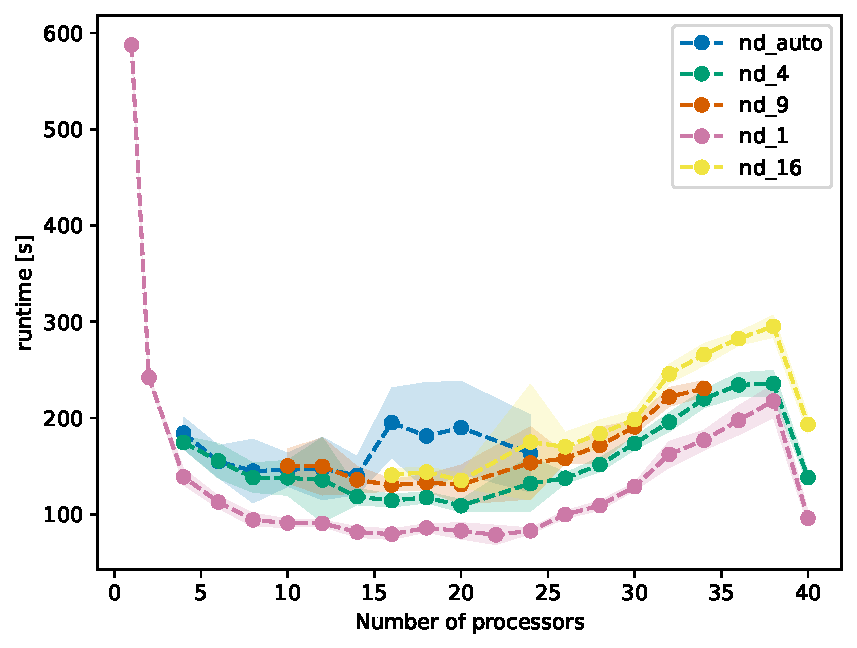
\includegraphics[width=\textwidth]{plots_scf/si_intel_mkl_bench_absolute.pdf}
\end{subfigure}
\label{fig:scaling_scf_nd_si}
\caption{Benchmark with linear algebra parallelization for the silicon benchmarking system}
\end{figure}

Fig. \ref{fig:scaling_scf_nd_si} shows the scaling behavior for different values of the parameter \texttt{nd}.
Here, nd\_auto means that no value for \texttt{nd} is specified so \QE automatically chooses the biggest square number smaller than the number of processors.
It is clearly shown that using linear algebra parallelization slows the calculation down significantly for the silicon system.

\begin{figure}[ht!]
\begin{subfigure}[b]{0.49\textwidth}
    \centering
    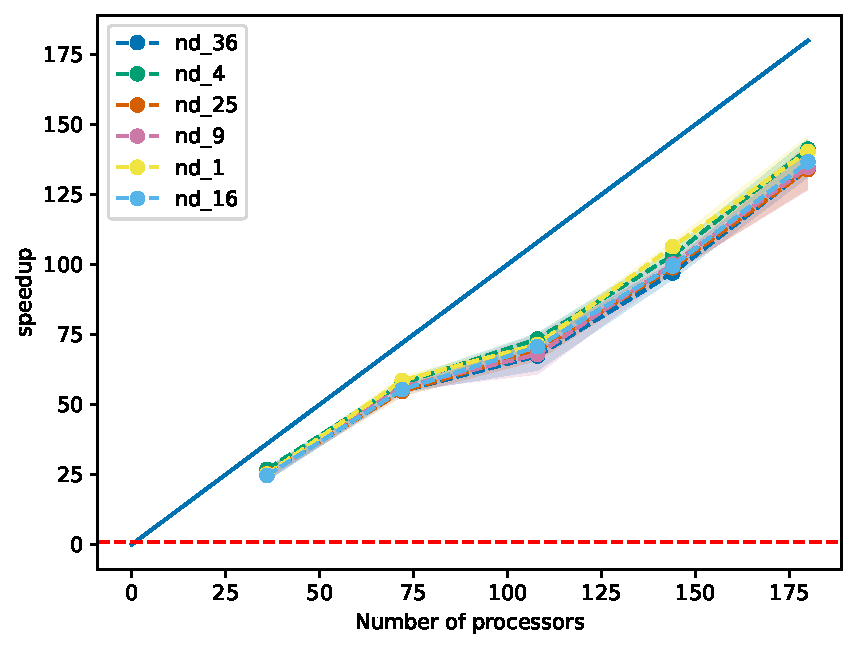
\includegraphics[width=\textwidth]{plots_scf/TaS2_intel_la_parallel_bench_speedup.pdf}
\end{subfigure}
\begin{subfigure}[b]{0.49\textwidth}
    \centering
    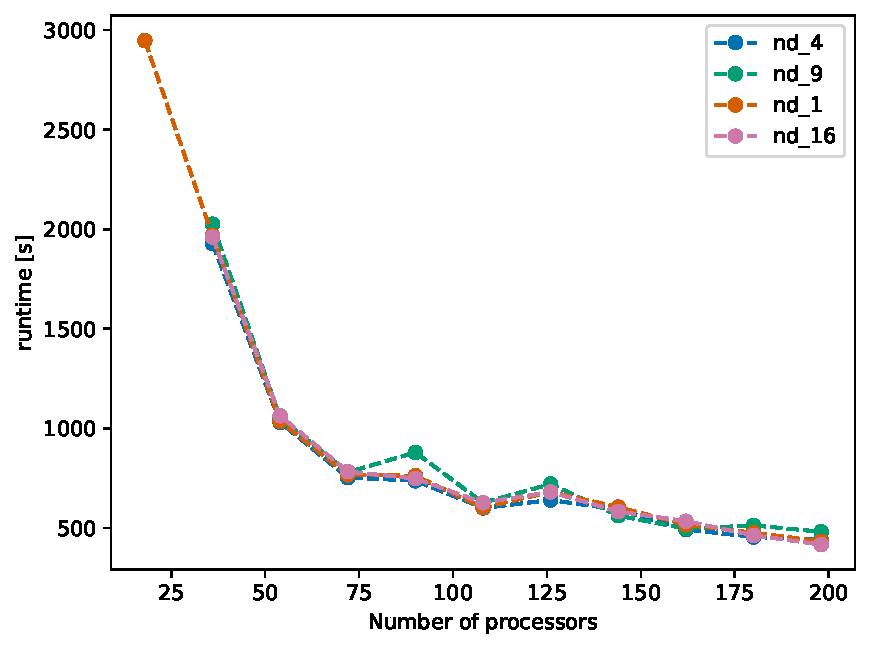
\includegraphics[width=\textwidth]{plots_scf/TaS2_intel_la_parallel_bench_absolute.pdf}
\end{subfigure}
\label{fig:scaling_scf_nd_tas2}
\caption{Benchmark with linear algebra parallelization for the TaS2 benchmarking system}
\end{figure}

Interestingly, this again is not reproduced for the more expensive TaS2 benchmarking system.
Fig. \ref{fig:scaling_scf_nd_tas2} shows a pretty much consistent times across all values for \texttt{nd}.

Those results are already hinted at in the \texttt{PWscf} user guide \cite{noauthor_pwscf_nodate}.
Here, in the guide for choosing parallelization parameters, using linear algebra parallelization is recommended when the number of \acrshort{kohn_sham} states is a few hundred or more.
The silicon system has 8 electrons and is as such described with 8 \gls{kohn_sham} states, the TaS2 system has 153 electrons, so \QE uses 92 \gls{kohn_sham} states (in case of metallic materials, the band occupation is smeared around the Fermi energy to avoid level crossings, so more \gls{kohn_sham} states than \(\frac{1}{2} * (\textrm{number of electrons})\) are needed to account for that).
Apparently, this number of \acrshort{kohn_sham} states is on the edge of linear algebra parallelization actually speeding up calculations.

\section{Comparison with calculations on the HLRN cluster}

\section{Conclusion: Parameters for optimal scaling}

\end{document}